\chapter{Métodos Ágeis}
\label{cap:metodosageis}
\section{Origem}
\par  Na década de 1990 com a decadência dos métodos clássicos de desenvolvimento de software - tal como o modelo Cascata, o qual propõe um rígido padrão de etapas sequenciais com maior ênfase no planejamento, considerado lento e burocrático com pouco espaço para alterações ou readaptações - novos modelos surgiram com o objetivo de obter maior interatividade entre o cliente e a produção, além de flexibilizar as etapas de planejamento e a validação do sistema.
\par Dentre esses modelos, os mais conhecidos e citados até hoje são: o desenvolvimento rápido de aplicações de 1994; processo unificado e Sistemas Dinâmicos de Método de Desenvolvimento (DSDM) de 1995; Scrum de 1996; \emph{Crystal Clear} e Programação Extrema (XP) - ambos de 1997.
\par Embora originados antes da publicação do Manifesto Ágil em 2001, são hoje coletivamente referidos como métodos ágeis, já que influenciaram diretamente na conceituação do manifesto.
\par Em fevereiro de 2001, dezessete desenvolvedores de software se reuniram no resort Snowbird em Utah (EUA), para discutir métodos leves de desenvolvimento. Na ocasião publicaram o Manifesto para Desenvolvimento Ágil de Software, documento que reúne os princípios e práticas desta metodologia. Mais tarde, algumas pessoas formaram a \emph{Agile Alliance}, uma organização sem fins lucrativos que promove o Desenvolvimento Ágil\footnote{Retirado de: \url{http://agilemanifesto.org/history.html} Acesso em: 12 set. 2016.}.
\section{Definição}
\par O Manifesto Ágil é baseado em doze princípios\footnote{Retirado de: \url{http://agilemanifesto.org/principles.html} Acesso em: 12 set. 2016.}:
\begin{enumerate}
  \item A satisfação do cliente é pela entrega antecipada e contínua do software funcional;
  \item Boas mundanças são sempre bem-vindas, mesmo que em desenvolvimento tardio;
  \item Novas funcionalidades devem ser entregues frequentemente (semanas em vez de meses);
  \item Uma cooperação estreita e diária entre cliente e desenvolvedor;
  \item Os projetos são construídos em torno de indivíduos motivados, entre os quais existe relação de confiança;
  \item A maneira mais eficiente e efetiva de transmitir informações é por conversas cara-a-cara;
  \item Softwares funcionais são a principal medida de progresso;
  \item Desenvolvimento sustentável, ou seja, produção em um ritmo constante;
  \item Atenção contínua à excelência técnica e bom design;
  \item Simplicidade em maximizar a quantidade de trabalho não feito;
  \item Melhores arquiteturas, requisitos e projetos emergem de equipes auto-organizadas;
  \item Regularmente, a equipe se reuni e reflete sobre como tornar-se mais eficaz, então se ajusta para o que foi acordado.
\end{enumerate}
\par Comparado à engenharia de software tradicional o Desenvolvimento Ágil de software tem como alvo principalmente sistemas complexos com características dinâmicas, ou seja, não-determinístico e não-linear, sendo que as estimativas precisas, os planos estáveis, e as previsões são muitas difíceis de se obter em estágios iniciais como na própria elaboração do projeto em si do produto. Isso resulta na necessidade de desenvolvimento e de planejamento evolutivo (\cite{Craig:04}).
\par Existem muitos modelos específicos de métodos ágeis. A maioria busca promover o trabalho em equipe, a colaboração e a adaptabilidade no processo em todo o ciclo de vida de desenvolvimento. Utiliza-se uma maior quantidade de ciclos em curtos períodos de tempo a fim de minimizar e parcelar o planejamento e estimativas. Desse modo, cada iteração envolve uma equipe multifuncional de trabalho para cada função necessária: planejamento, análise, projeto, desenvolvimento, testes unitários e testes de aceitação. No final da iteração é demonstrado para as partes interessadas, cliente, o que foi desenvolvido no processo. Por fim, isto minimiza o risco global de erros e permite que o produto se adapte às mudanças rapidamente.
\par Independente do método ágil seguido, cada equipe deve incluir um representante do cliente no processo. No caso do Scrum, essa é a função do ``proprietário do produto'', por exemplo. Por compromisso, este colaborador se coloca disponível para os desenvolvedores, respondendo questões durante cada iteração. A inclusão deste representante otimiza o retorno de investimento e garante o alinhamento com as necessidades do cliente.
\par Outra característica comum deste tipo de metodologia é o \emph{stand-up} diário. Em uma breve sessão, os membros da equipe comunicam uns aos outros o que eles fizeram no dia anterior sobre as tarefas relacionadas ao ciclo vigente, o que eles pretendem fazer, e quaisquer obstáculos ou impedimentos para continuar ou finalizar a tarefa do dia para a interação em questão.
\par Diferentes ferramentas e técnicas específicas, tais como a integração contínua, os testes de unidade automatizado, a programação em pares, o desenvolvimento orientado a testes, os padrões de projeto, o \emph{Domain-Driven Design}, a refatoração de código entre outras, são frequentemente utilizadas para melhorar a qualidade e aumentar a agilidade de produção.

\section{Métodos Ágeis específicos}
\subsection{Scrum}
\par Scrum é um dos arcabouços mais populares hoje de Desenvolvimento Ágil de Software. Um princípio chave do Scrum é o reconhecimento de que, durante o desenvolvimento do produto, os clientes podem mudar de opinião sobre o que eles querem e precisam, muitas vezes chamado de volatilidade de requisitos, pois desafios imprevistos normalmente não podem ser tratados de forma preventiva ou planejados tradicionalmente.
\par O arcabouço propõe inicialmente três papéis principais para divisão e organização da equipe de trabalho:
\begin{itemize}
\item\textbf{Product Owner (Dono do Produto):}
\par Representa as partes interessadas do produto, ou seja, é a voz do cliente, é responsável por garantir que a equipe agregue valor ao negócio. Passa a maior parte do seu tempo em comunicação com as partes interessadas, mas não aponta necessariamente como a equipe deve chegar à uma solução técnica.
\par Este papel é equivalente a ``representante do cliente'', papel em alguns outros emph{frameworks} ágeis, como Programação Extrema (XP).
\item\textbf{Scrum Master (Mestre Scrum):}
\par Responsável direto pela solução de possíveis impedimentos da equipe para entregar as metas de produtos e resultados, seja impedimentos estruturais ou pessoais da equipe.
\par \emph{Scrum Master} não é um líder de equipe ou gerente de projeto tradicional mas age como um mediador entre a equipe e quaisquer influências que a distraem.
\par Ele é o responsável por garantir que o Scrum seja seguido, ajudando a equipe a seguir os processos acordados e incentivando a melhorar.
\par O papel também tem sido referido como um ``facilitador da equipe'' ou ``servo-líder'' para reforçar estas duas perspectivas.
\item\textbf{Development Team (Equipe de Desenvolvimento):}
\par A Equipe de Desenvolvimento é responsável pela entrega de incrementos do produto no final de cada Sprint (ciclo de interação).
\par A equipe é composta de indivíduos que fazem o trabalho real (analisar, projetar, desenvolver, testar, documentar, etc.). As equipes de desenvolvimento são multifuncionais, com todas as habilidades necessárias para criar um produto.
\end{itemize}
\par O ciclo de interação chamado \emph{sprint} é a unidade básica do desenvolvimento em Scrum. É restrito a uma duração específica fixada antecipadamente, normalmente entre uma semana e um mês, com duas semanas sendo o mais comum.
\par Cada \emph{sprint} começa com um evento de planejamento(\emph{Sprint Planning}), que visa definir a lista de objetivos à serem tratados ou implementados nesse ciclo(\emph{Sprint Backlog}). Por fim, termina com uma revisão(\emph{Sprint Review}), que analisa os progressos realizados para mostrar aos interessados, além disso é debatido as lições e melhorias a serem aplicadas para as próximas interações(\emph{Sprint Retrospective}).
\begin{figure}[!htb]
\centering
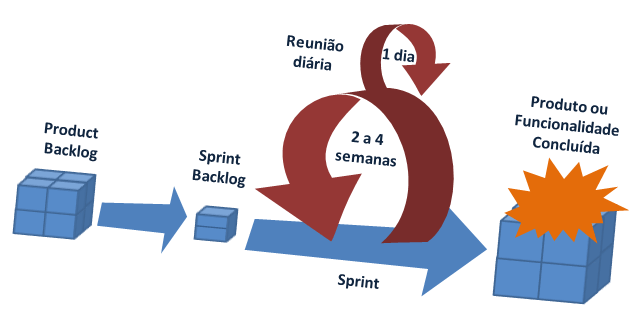
\includegraphics[width=11cm]{figuras/scrum_process}
\caption{\label{fig:scrum_process}O ciclo interativo Sprint.}
\end{figure}
\subsection{Test Driven Development (TDD)}
\par TDD é um processo de desenvolvimento de software que se baseia na repetição de um ciclo de desenvolvimento muito curto: requisitos são transformados em casos de teste específico, em seguida, o software é aprimorado somente para passar no teste específico, mas todos os teste são refeitos a cada interação. Este processo também é chamado de ciclo \emph{Red-Green-Refactor}.
\par Cada novo recurso a ser implementado começa com o desenvolvimento de um teste que define uma função ou melhorias de uma função, o mais preciso e sucinto possível. A nova funcionalidade agora é implementada com objetivo em passar neste novo teste. Esta é principal característica do TDD, que em contrapartida aos demais métodos em que os testes são criados após a implementação da nova função.
\par Ao passar no novo teste todo código é então também submetido aos testes anteriores, se passar em todos, o programador possui uma maior garantia da integralidade do novo código, ou seja, atende aos requisitos de teste e não degrada quaisquer outros recursos existentes. Se não passar em um ou mais dos testes anteriores o novo código então deve ser ajustado até que passe em todos os testes. Essa etapa é chamada de refatoração.
\begin{figure}[!htb]
\centering
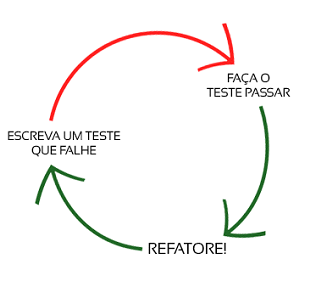
\includegraphics[width=8cm]{figuras/red_green}
\caption{\label{fig:red_green}O ciclo \emph{Red-Green-Refactor}.}
\end{figure}
\subsection{Continuous Integration (CI)}
\par Integração contínua é um dos pilares da agilidade, garantindo que todo o sistema funcione a cada interação de forma coesa, mesmo que sua equipe seja grande e diversas partes do código estejam sendo alteradas ao mesmo tempo, isso traz um \emph{feedback} diário do desenvolvimento.
\par Essa integração é alinhada diretamente com o conceito de TDD em que cada ciclo é aplicado um conjunto de testes e verificações de integração entre as partes produzidas, além dos testes técnicos da aplicação.
\par A parte crucial desse processo dentro do conceito de CI é o uso de alguma sistema de controle de versão, estabelecendo como compartilhar informações de maneira sucinta e objetiva, mantendo a última versão do produto válida e ainda saber quem ou qual parte de equipe fez cada alteração, prevenindo desperdício de desenvolvimento, seja por duplicidade ou refatoração direta.
\par Existe um conjunto de ferramentas para controle de versão centralizado, entre elas temos o \emph{CVS}, \emph{Subversion}, \emph{Git}, entre outros. O controle de versão, gerencia não apenas o código do produto, mas como também a documentação, \emph{scripts} de teste, arquivos de layout e configuração, entre outros. Além disso, e mais importante, é possível criar linhas alternativas de desenvolvimento do produto, chamado de \emph{branches}.
\par O sistema funciona basicamente da seguinte forma: o desenvolvedor faz seu código, efetua um \emph{build} antes de interagir com a base principal do que já foi feito e testado. Os \emph{builds} são posteriormente integrados à base por meio de sincronização, o que é feito sob testes e padrões de produção. Essa prática permite uma divisão coesa das tarefas a serem desenvolvidas, eliminando a necessidade de que toda equipe saiba exatamente como cada parte do produto foi ou será feita, trazendo uma visão de linha de montagem: cada desenvolvedor deve saber como fazer especificamente a sua parte, porém consistente à quem deve recorrer caso tenha problemas com outras partes do produto.
\subsection{Kanban}
\par \emph{Kanban} é um termo de origem japonesa, significa literalmente ``cartão'' ou ``sinalização''. O conceito foi relacionado com a utilização de cartões para indicar o andamento dos fluxos de produção em empresas de fabricação em série, hoje popularmente utilizado em Métodos Ágeis. Os cartões são organizados sob uma determinada etapa do processo de implementação, por exemplo, ``para executar'', ``em andamento'' ou ``finalizado''.
\par A empresa japonesa de automóveis \emph{Toyota} foi a responsável pela introdução desse método devido a necessidade de manter um eficaz funcionamento do sistema de produção em série.
\begin{figure}[!htb]
\centering
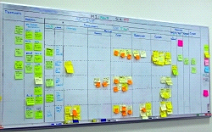
\includegraphics[width=8cm]{figuras/kanban_exemplo}
\caption{\label{fig:kanban_exemplo}Exemplo de um quadro de \emph{Kanban}.}
\end{figure}

\section{Um contraponto: O modelo Cascata}
    \par O modelo Cascata, algumas vezes chamado de ciclo de vida clássico, sugere uma abordagem sequencial e sistemática para o desenvolvimento de software, começando com o levantamento de necessidades por parte do cliente, avançando para as fases de planejamento, modelagem, construção, emprego e culminando no suporte contínuo do software concluído (figura \ref{fig:waterfall}). (\cite{pressman:11})
    \par Segundo (\cite{pressman:11}), o modelo em cascata foi o primeiro paradigma de desenvolvimento criado pela Engenharia de Software, que teve sua essência retirada de outras áreas da Engenharia.
\begin{figure}[htb]
\centering
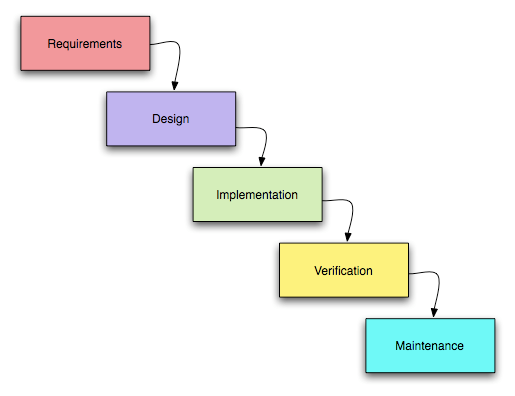
\includegraphics[width=10cm]{figuras/waterfall}
\caption{\label{fig:waterfall}O Modelo Cascata.}
\end{figure}
	\par As fases do Modelo são:
\begin{itemize}
\item \emph{ Requerimentos:} Realizar a análise de requisitos do projeto.
\item \emph{ Design de Projeto:}  Focando na estrutura de dados, arquitetura do software, detalhes procedurais e caracterização das interfaces é formulado um documento de forma a apresentar os requerimentos de uma forma que possa ser interpretado pelos programadores.
\item \emph{ Implementação:} Etapa da codificação do projeto propriamente dita.
\item \emph{  Verificação: } Etapa para teste do produto visando eliminar qualquer \emph{bug} que possa ter passado despercebido e refinar a lógica interna do software caso necessário.
\item \emph{ Manutenção: } Etapa para instalação do sistema no cliente, configuração de servidores, etc.
\end{itemize}

\par Uma das grandes críticas dessa abordagem é que dificilmente um desenvolvimento de software segue todas as etapas da forma como o modelo propõe  e nem sempre o cliente sabe definir bem os requisitos antes de ver o software funcionando, resultando em tempo e desenvolvimento desperdiçado em funcionalidades que não resolvem o problema.(\cite{pressman:11})
\par Mudanças tardias no escopo do projeto encarecem o custo total e poderiam ter sido evitadas e contornadas de maneira mais satisfatória em um modelo com um processo de desenvolvimento iterativo \footnote{ Fonte: Wikipedia - Waterfall Model \url {https://en.wikipedia.org/wiki/Waterfall_model} Acesso em: 12 set. 2016.}.
\par O Desenvolvimento Ágil tem pouco em comum com o Modelo em Cascata. Na visão de alguns este modelo é desacreditado, apesar de ser um modelo de uso comum. O modelo em Cascata é uma das metodologias com maior ênfase no planejamento, seguindo seus passos a partir da captura dos requisitos, análise, projeto, codificação e testes em uma seqüência pré-planejada e restrita. \footnote {Fonte: Wikipedia - Desenvolvimento Ágil de Software: \url{https://pt.wikipedia.org/wiki/Desenvolvimento_\%C3\%A1gil_de_software#Compara.C3.A7.C3.A3o_com_o_modelo_em_cascata} Acesso em: 12 set. 2016.}
